%%%%%%%%%%%%%%%%%%%%%%%%%%%%%%%%%%%%%%%%%
% Beamer Presentation
% LaTeX Template
% Version 1.0 (10/11/12)
%
% This template has been downloaded from:
% http://www.LaTeXTemplates.com
%
% License:
% CC BY-NC-SA 3.0 (http://creativecommons.org/licenses/by-nc-sa/3.0/)
%
%%%%%%%%%%%%%%%%%%%%%%%%%%%%%%%%%%%%%%%%%

%----------------------------------------------------------------------------------------
%	PACKAGES AND THEMES
%----------------------------------------------------------------------------------------

\documentclass{beamer}

\mode<presentation> {

% The Beamer class comes with a number of default slide themes
% which change the colors and layouts of slides. Below this is a list
% of all the themes, uncomment each in turn to see what they look like.

%\usetheme{default}
%\usetheme{AnnArbor}
%\usetheme{Antibes}
%\usetheme{Bergen}
%\usetheme{Berkeley}
%\usetheme{Berlin}
%\usetheme{Boadilla}
%\usetheme{CambridgeUS}
%\usetheme{Copenhagen}
%\usetheme{Darmstadt}
%\usetheme{Dresden}
%\usetheme{Frankfurt}
%\usetheme{Goettingen}
%\usetheme{Hannover}
%\usetheme{Ilmenau}
%\usetheme{JuanLesPins}
%\usetheme{Luebeck}
\usetheme{Madrid}
%\usetheme{Malmoe}
%\usetheme{Marburg}
%\usetheme{Montpellier}
%\usetheme{PaloAlto}
%\usetheme{Pittsburgh}
%\usetheme{Rochester}
%\usetheme{Singapore}
%\usetheme{Szeged}
%\usetheme{Warsaw}

% As well as themes, the Beamer class has a number of color themes
% for any slide theme. Uncomment each of these in turn to see how it
% changes the colors of your current slide theme.

%\usecolortheme{albatross}
%\usecolortheme{beaver}
%\usecolortheme{beetle}
%\usecolortheme{crane}
%\usecolortheme{dolphin}
%\usecolortheme{dove}
%\usecolortheme{fly}
%\usecolortheme{lily}
%\usecolortheme{orchid}
%\usecolortheme{rose}
%\usecolortheme{seagull}
%\usecolortheme{seahorse}
%\usecolortheme{whale}
%\usecolortheme{wolverine}

%\setbeamertemplate{footline} % To remove the footer line in all slides uncomment this line
%\setbeamertemplate{footline}[page number] % To replace the footer line in all slides with a simple slide count uncomment this line

%\setbeamertemplate{navigation symbols}{} % To remove the navigation symbols from the bottom of all slides uncomment this line
}

\usepackage{graphicx} % Allows including images
\usepackage{booktabs} % Allows the use of \toprule, \midrule and \bottomrule in tables

%----------------------------------------------------------------------------------------
%	TITLE PAGE
%----------------------------------------------------------------------------------------

\title[LNG 230/SPV 221 Language Acquisition]{Word Acquisition II} % The short title appears at the bottom of every slide, the full title is only on the title page

\author{Xiaomeng Ma} % Your name
\institute[Graduate Center, CUNY] % Your institution as it will appear on the bottom of every slide, may be shorthand to save space
{Graduate Center, CUNY \\ % Your institution for the title page
\medskip
\textit{xma3@gradcenter.cuny.edu} % Your email address
}
\date{October 1, 2018} % Date, can be changed to a custom date

\begin{document}

\begin{frame}
\titlepage % Print the title page as the first slide
\end{frame}


%----------------------------------------------------------------------------------------
%	PRESENTATION SLIDES
%----------------------------------------------------------------------------------------

%------------------------------------------------
\section{First Section} % Sections can be created in order to organize your presentation into discrete blocks, all sections and subsections are automatically printed in the table of contents as an overview of the talk
%------------------------------------------------

\subsection{Subsection Example} % A subsection can be created just before a set of slides with a common theme to further break down your presentation into chunks

\begin{frame}{Word Acquisition}
\begin{itemize}
\item Difficulties in Word Acquisition
\pause 
\begin{itemize}
    \item Reference
    \item Extension
\end{itemize}
\item Constraints Theory
\begin{itemize}
    \item whole item assumption
    \item mutual exclusivity assumption 
    \item developmental lexcial framework
\end{itemize}
\end{itemize}
\end{frame}
%------------------------------------------------
\begin{frame}
\frametitle{Other Routes to Word Learning}
\textbf{Do we need innate linguistic biases? What other factors are there?}
\begin{itemize}
\item Social-pragmatic account: 
\\ Children do not need innate linguistic constraints. Children pay attention to "social clues" to learn the meaning of new words. 
\begin{itemize}
    \item Joint Attention
    \\ https://www.youtube.com/watch?v=UUwGLDeYN8c
    \pause
    \item Communicative Intent
\end{itemize}
\end{itemize}
\end{frame}
%------------------------------------------------
\begin{frame}
\frametitle{Evidence FOR social-pragmatic account}
Baldwin 1993b 
\begin{itemize}
\item Participants: 19-20 month old infants
\item Children and researcher were playing with different toys
\item Experiment group: Researcher waited until joint attention were given on children's toy, then named the toy \textit{Toma}
\item Control group: Researcher named the toy that the children were not paying attention to \textit{Toma}
\item Results: In both group, the children successfully found \textit{Toma}
\item Implication: Children are aware that it is the speaker’s focus of attention, not their own, that matters when trying to learn the meaning of a new word.
\end{itemize}
\end{frame}
%------------------------------------------------
\begin{frame}
\frametitle{Evidence for social-pragmatic account}
Tomasello and Akhtar (1995)
\begin{itemize}
\item Participants: two year old children
\item Researchers created a device that had a toy that spun around a turntable
\item Action Highlighted: Researcher prepared the device, gaze shifted between device and child, "widget it"
\item Object Highlighted: Researcher picked up the toy and gaze shifted between the toy and the child "widget"
\item "Can you show me \textit{Widget it?} \textit{Widget?}"
\end{itemize}
\end{frame}
%------------------------------------------------
\begin{frame}
\frametitle{Problems with social-pragmatic account}
\begin{itemize}
\item Acquisition could take place without social cues
\begin{itemize}
    \item Children early than 19 months (haven't developed joint attention) also learn words
    \item Autistic children (who have impaired joint attention) also learn words
\end{itemize}
\pause
\item We don't nee social pragmatic account
\begin{itemize}
    \item "Gazzer experiment"
    \item For: children used communicative intent to apply the name "gazzer"
    \item Against: "gazzer" is contextually novel
\end{itemize}
\end{itemize}
\end{frame}
%------------------------------------------------
\begin{frame}
\frametitle{Attentional Learning Account}
\begin{itemize}
\item Associative Learning Ability 
\item  “general processes of perceiving, remembering, and attending ... may be sufficient in and of themselves to create children’s smart word interpretations” (Samuelson & Smith, 1998, p. 95)
\end{itemize}
\end{frame}
%------------------------------------------------
\begin{frame}
\frametitle{Syntactic Bootstrapping}
\textit{does verb acquisition require knowledge of syntax}
\begin{itemize}
\item Verbs are more difficult to learn than nouns 
\begin{itemize}
    \item Verb association is difficult
    \item Verb also has conjugations
\end{itemize}
\item that children exploit (possibly universal) mappings between meaning (semantics) and syntax to learn verbs through constraints of sentence types
\item Syntactic Bootstrapping: 
\end{itemize}
\end{frame}
%------------------------------------------------
\begin{frame}
\frametitle{Evidence FOR syntactic bootstrapping}
Naigles (1990)
\begin{itemize}
    \item Fact: People have an unconscious tendency to look at things that are being spoken about.
    \item Participants: 24 month old babies
    \item "The duck is gorping the bunny." vs "The duck and bunny are gorping."
    \item \begin{figure}
        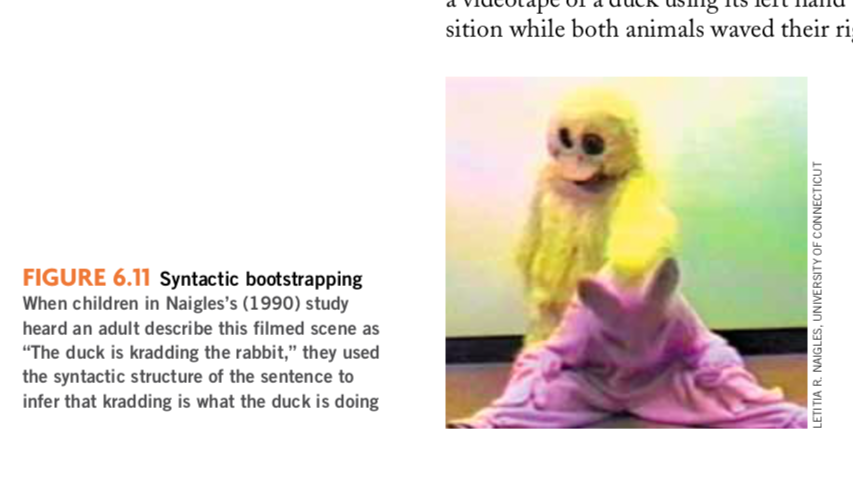
\includegraphics[height = 5cm, width = \textwidth]{111111.png}
    \end{figure}
\end{itemize}
\end{frame}
%------------------------------------------------
\begin{frame}
\frametitle{Evidence AGAINST syntactic bootstrapping}
\begin{itemize}
    \item Is syntax really NECESSARY for word leanring?
    \begin{itemize}
        \item Syntax acquisition is slower
        \item Syntax is only available to older children (2y/o)
        \item Sometimes failed, e.g giving and receiving (Fisher 1996)
    \end{itemize}
    \pause
    \item Syntactic bootstrapping would actually hinder verb learning
    \begin{itemize}
        \item Passive sentences
        \item problematic case in Saliba
    \end{itemize}
\end{itemize}
\end{frame}
%------------------------------------------------
\begin{frame}
\frametitle{Emergentist Coalition Model (ECM)}
 constraints, socio- pragmatic abilities, cognitive processing abilities and syntax, do we need an integrated account that takes some, or all, of them into account?
\begin{itemize}
\item Emergentist Coalition Model: a hybrid account that is sensitive to the multiple strategies children use to break the word barrier and to move from being novice to expert learners (Hollich et al., 2000, p. 17).
\pause
\item Children are sensitive to cues in word learning.
\item Children compute the reliability of different cues across different situations and rely on different cues to learn words
\item Constraints on word learning emerge from the developmental process itself.
\end{itemize}
\end{frame}


\end{document}